\documentclass[dvips, lscape]{foils}
%\documentclass[dvips, french]{slides}
\textwidth 18.5cm
\textheight 25cm 
\topmargin -1cm 
\oddsidemargin  -1cm 
\evensidemargin  -1cm

% Maths
\usepackage{amsfonts, amsmath, amssymb}

\newcommand{\coefbin}[2]{\left( 
    \begin{array}{c} #1 \\ #2 \end{array} 
  \right)}
\newcommand{\Bcal}{\mathcal{B}}
\newcommand{\Ccal}{\mathcal{C}}
\newcommand{\Dcal}{\mathcal{D}}
\newcommand{\Ecal}{\mathcal{E}}
\newcommand{\Gcal}{\mathcal{G}}
\newcommand{\Mcal}{\mathcal{M}}
\newcommand{\Ncal}{\mathcal{N}}
\newcommand{\Pcal}{\mathcal{P}}
%\newcommand{\Qcal}{\mathcal{Q}}
\newcommand{\Lcal}{\mathcal{L}}
\newcommand{\Tcal}{\mathcal{T}}
\newcommand{\Ucal}{\mathcal{U}}
\newcommand{\alphabf}{\text{\mathversion{bold}{$\alpha$}}}
\newcommand{\betabf}{\text{\mathversion{bold}{$\beta$}}}
\newcommand{\gammabf}{\text{\mathversion{bold}{$\gamma$}}}
\newcommand{\mubf}{\text{\mathversion{bold}{$\mu$}}}
\newcommand{\thetabf}{\text{\mathversion{bold}{$\theta$}}}
\newcommand{\Pibf}{\text{\mathversion{bold}{$\Pi$}}}
\newcommand{\psibf}{\text{\mathversion{bold}{$\psi$}}}
\newcommand{\Sigmabf}{\text{\mathversion{bold}{$\Sigma$}}}
\newcommand{\taubf}{\text{\mathversion{bold}{$\tau$}}}
\newcommand{\Cbf}{{\bf C}}
\newcommand{\Ebf}{{\bf E}}
\newcommand{\Gbf}{{\bf G}}
\newcommand{\Hbf}{{\bf H}}
\newcommand{\Ibf}{{\bf I}}
\newcommand{\mbf}{{\bf m}}
\newcommand{\Obf}{{\bf 0}}
\newcommand{\Rbf}{{\bf R}}
\newcommand{\Sbf}{{\bf S}}
\newcommand{\Tbf}{{\bf T}}
\newcommand{\Ubf}{{\bf U}}
\newcommand{\Vbf}{{\bf V}}
\newcommand{\xbf}{{\bf x}}
\newcommand{\Xbf}{{\bf X}}
\newcommand{\Ybf}{{\bf Y}}
\newcommand{\Zbf}{{\bf Z}}
\newcommand{\Esp}{{\mathbb E}}
\newcommand{\Var}{{\mathbb V}}
\newcommand{\Cov}{{\mathbb C}\text{ov}}
\newcommand{\Ibb}{{\mathbb I}}
\newcommand{\Rbb}{\mathbb{R}}

% sommes
\newcommand{\sumk}{\sum_k}
\newcommand{\sumt}{\sum_{t \in I_k}}
\newcommand{\sumth}{\sum_{t=t_{k-1}^{(h)}+1}^{t_k^{(h)}}}
\newcommand{\sump}{\sum_{p=1}^{P}}
\newcommand{\suml}{\sum_{\ell=1}^{P}}
\newcommand{\sumtau}{\sum_k \hat{\tau}_{kp}}

% Couleur et graphiques
\usepackage{color}
\usepackage{graphics}
\usepackage{epsfig} 
\usepackage{pstcol}

% Texte
\usepackage{lscape}
\usepackage{../../../../Latex/fancyheadings, rotating, enumerate}
%\usepackage[french]{babel}
\usepackage[latin1]{inputenc}
\definecolor{darkgreen}{cmyk}{0.5, 0, 0.5, 0.5}
\definecolor{orange}{cmyk}{0, 0.6, 0.8, 0}
\definecolor{jaune}{cmyk}{0, 0.5, 0.5, 0}
\newcommand{\textblue}[1]{\textcolor{blue}{#1}}
\newcommand{\textred}[1]{\textcolor{red}{#1}}
\newcommand{\textgreen}[1]{\textcolor{green}{ #1}}
\newcommand{\textlightgreen}[1]{\textcolor{green}{#1}}
%\newcommand{\textgreen}[1]{\textcolor{darkgreen}{#1}}
\newcommand{\textorange}[1]{\textcolor{orange}{#1}}
\newcommand{\textyellow}[1]{\textcolor{yellow}{#1}}
\newcommand{\refer}[2]{{\sl #1}}
\newcommand{\emphase}[1]{\textblue{\sl #1}}

% Sections
%\newcommand{\chapter}[1]{\centerline{\LARGE \textblue{#1}}}
% \newcommand{\section}[1]{\centerine{\Large \textblue{#1}}}
% \newcommand{\subsection}[1]{\noindent{\Large \textblue{#1}}}
% \newcommand{\subsubsection}[1]{\noindent{\large \textblue{#1}}}
% \newcommand{\paragraph}[1]{\noindent {\textblue{#1}}}
% Sectionsred
\newcommand{\chapter}[1]{
  \addtocounter{chapter}{1}
  \setcounter{section}{0}
  \setcounter{subsection}{0}
%  {\centerline{\LARGE \textblue{\arabic{chapter} - #1}}}
  {\centerline{\LARGE \textblue{#1}}}
  }
\newcommand{\section}[1]{
  \addtocounter{section}{1}
  \setcounter{subsection}{0}
%  {\centerline{\Large \textblue{\arabic{chapter}.\arabic{section} - #1}}}
  {\centerline{\Large \textblue{#1}}}
  }
\newcommand{\subsection}[1]{
  \addtocounter{subsection}{1}
  {\noindent{\large \textblue{#1}}}
  }
% \newcommand{\subsection}[1]{
%   \addtocounter{subsection}{1}
%   {\noindent{\large \textblue{\arabic{chapter}.\arabic{section}.\arabic{subsection} - #1}}}
%   }
\newcommand{\paragraph}[1]{\noindent{\textblue{#1}}}

%%%%%%%%%%%%%%%%%%%%%%%%%%%%%%%%%%%%%%%%%%%%%%%%%%%%%%%%%%%%%%%%%%%%%%
%%%%%%%%%%%%%%%%%%%%%%%%%%%%%%%%%%%%%%%%%%%%%%%%%%%%%%%%%%%%%%%%%%%%%%
%%%%%%%%%%%%%%%%%%%%%%%%%%%%%%%%%%%%%%%%%%%%%%%%%%%%%%%%%%%%%%%%%%%%%%
%%%%%%%%%%%%%%%%%%%%%%%%%%%%%%%%%%%%%%%%%%%%%%%%%%%%%%%%%%%%%%%%%%%%%%
\begin{document}
%%%%%%%%%%%%%%%%%%%%%%%%%%%%%%%%%%%%%%%%%%%%%%%%%%%%%%%%%%%%%%%%%%%%%%
%%%%%%%%%%%%%%%%%%%%%%%%%%%%%%%%%%%%%%%%%%%%%%%%%%%%%%%%%%%%%%%%%%%%%%
%%%%%%%%%%%%%%%%%%%%%%%%%%%%%%%%%%%%%%%%%%%%%%%%%%%%%%%%%%%%%%%%%%%%%%
%%%%%%%%%%%%%%%%%%%%%%%%%%%%%%%%%%%%%%%%%%%%%%%%%%%%%%%%%%%%%%%%%%%%%%
\landscape
\newcounter{chapter}
\newcounter{section}
\newcounter{subsection}
\setcounter{chapter}{0}
\headrulewidth 0pt 
\pagestyle{fancy} 
\cfoot{}
\rfoot{\begin{rotate}{90}{
      \hspace{1cm} \tiny S. Robin: Analysis of mutiple CGH arrays
      }\end{rotate}}
\rhead{\begin{rotate}{90}{
      \hspace{-.5cm} \tiny \thepage
      }\end{rotate}}

%%%%%%%%%%%%%%%%%%%%%%%%%%%%%%%%%%%%%%%%%%%%%%%%%%%%%%%%%%%%%%%%%%%%%%
%%%%%%%%%%%%%%%%%%%%%%%%%%%%%%%%%%%%%%%%%%%%%%%%%%%%%%%%%%%%%%%%%%%%%%
\begin{center}
  \textblue{\LARGE Statistical Analysis of CGH Arrays}

   \vspace{1cm}
   {\large F. Picard, E. Lebarbier, E. Budinska, \underline{S. Robin}} \\
   robin@inapg.inra.fr

   {UMR AgroParisTech  / INRA, Paris} \\
   {Math�matique et Informatique Appliqu�es}
   
    \vspace{1cm}
    {Coimbra, WSGP, \today}
\end{center}

%\vspace{2cm}
\paragraph{Outline}

1 - Microarray CGH technology 

2 - Single array analysis  

3 - Multiple arrays analysis

4 - Development: Clustering segments

%%%%%%%%%%%%%%%%%%%%%%%%%%%%%%%%%%%%%%%%%%%%%%%%%%%%%%%%%%
%%%%%%%%%%%%%%%%%%%%%%%%%%%%%%%%%%%%%%%%%%%%%%%%%%%%%%%%%%%%%
\newpage
\chapter{Microarray CGH technology}
%%%%%%%%%%%%%%%%%%%%%%%%%%%%%%%%%%%%%%%%%%%%%%%%%%%%%%%%%%%%%
\bigskip\bigskip
%%%%%%%%%%%%%%%%%%%%%%%%%%%%%%%%%%%%%%%%%%%%%%%%%%%%%%%%%%%%%
\section{Looking for chromosomal alterations}
%%%%%%%%%%%%%%%%%%%%%%%%%%%%%%%%%%%%%%%%%%%%%%%%%%%%%%%%%%%%%
\bigskip
\paragraph{At the chromosomic scale: e.g. trisomy.} Experimental tool
= \emphase{Karyotype}
$$
\epsfig{file = ../Figures/Karyotype.ps, clip=,
  bbllx=158, bblly=560, bburx=452, bbury=778, scale=1.2}
$$

%%%%%%%%%%%%%%%%%%%%%%%%%%%%%%%%%%%%%%%%%%%%%%%%%%%%%%%%%%%%%
\newpage
\paragraph{At a lower scale: within chromosome.} Experimental tool =
Comparative Genomic Hybridization (\emphase{CGH}).  
$$
\vspace{-1cm}
\epsfig{file = ../Figures/principe_CGH.eps, clip=,
  bbllx=0, bblly=41, bburx=700, bbury=478, scale=0.8}
$$
\emphase{Resolution $\sim$ 100kb.}

%%%%%%%%%%%%%%%%%%%%%%%%%%%%%%%%%%%%%%%%%%%%%%%%%%%%%%%%%%%%%
\newpage
\section{Microarray technology}
%%%%%%%%%%%%%%%%%%%%%%%%%%%%%%%%%%%%%%%%%%%%%%%%%%%%%%%%%%
\noindent Same technology as for gene expression but cDNA (retro-transcripted
from RNA) is replaced by \emphase{genomic DNA} (for both targets and
probes): \\ 
\centerline{ \epsfig{file =
    /RECHERCHE/EXPRESSION/EXPOSES/Figures/MicroarrayTech.ps,
    width=20cm} }

%%%%%%%%%%%%%%%%%%%%%%%%%%%%%%%%%%%%%%%%%%%%%%%%%%%%%%%%%%%%%
\newpage
\section{CGH profile }
%%%%%%%%%%%%%%%%%%%%%%%%%%%%%%%%%%%%%%%%%%%%%%%%%%%%%%%%%%%%%
\vspace{-0.5cm}
$$
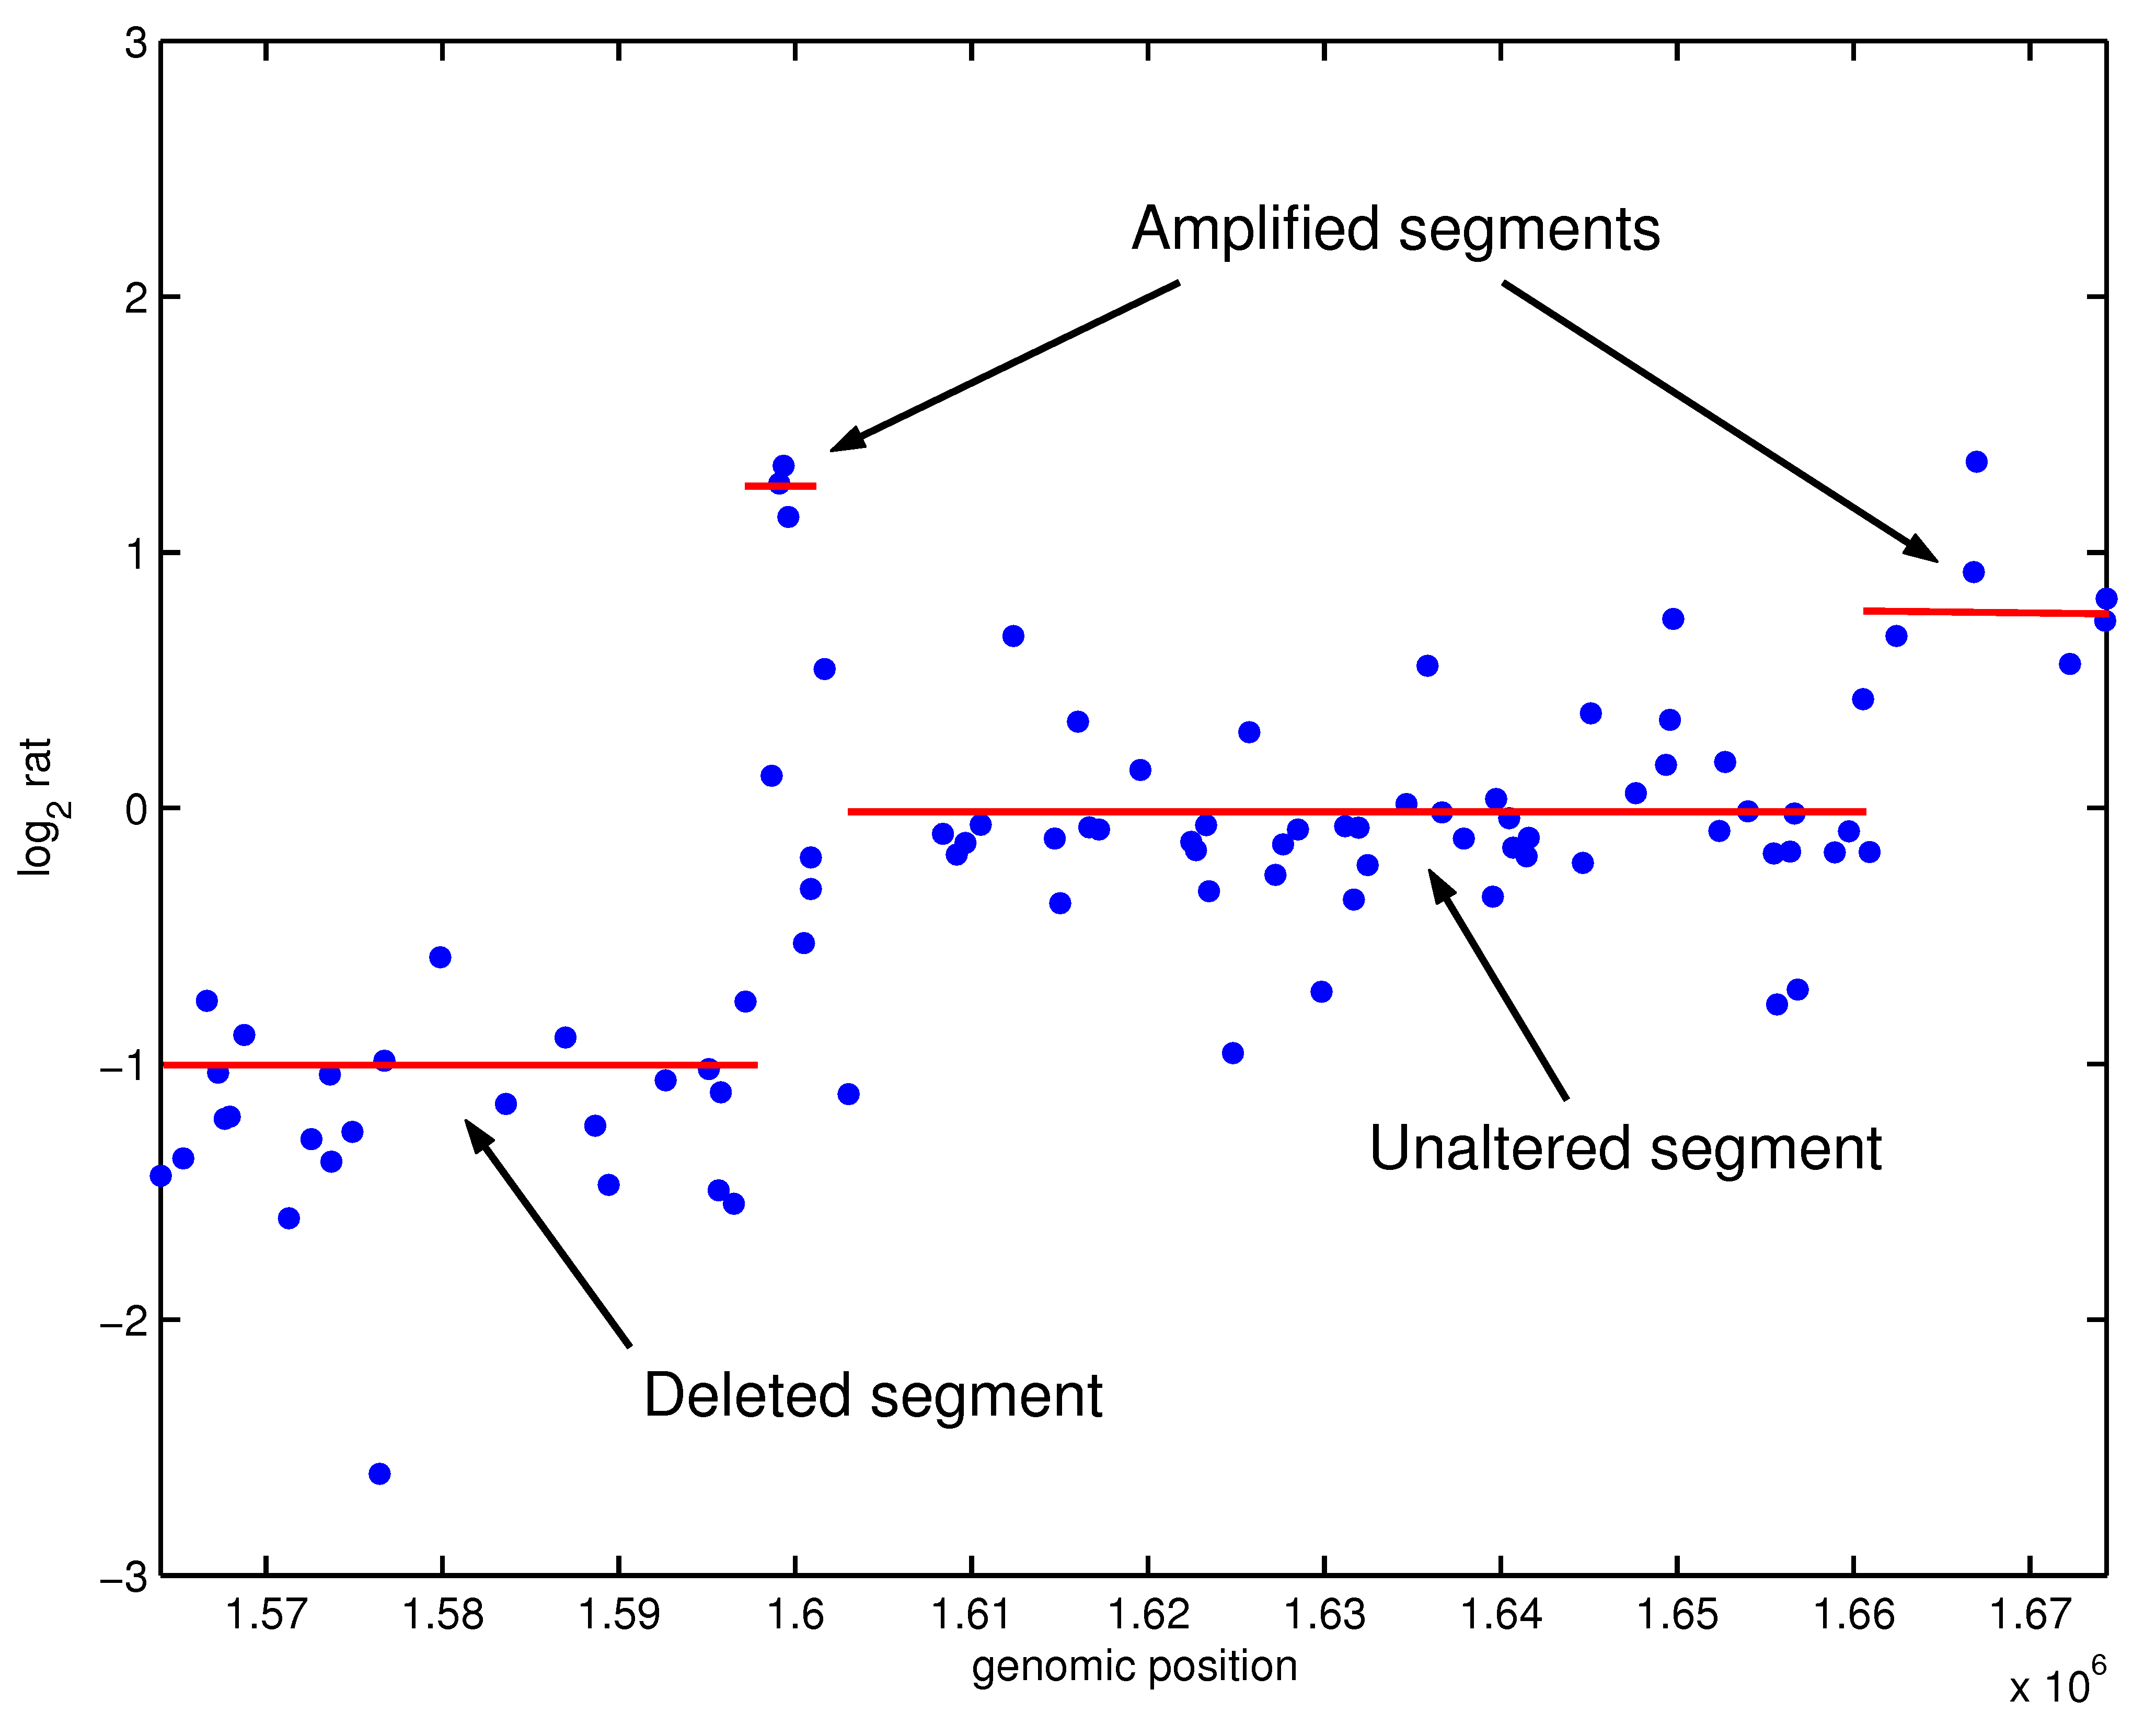
\epsfig{file = ../Figures/profile_example.eps, clip=,
  bbllx=60, bblly=196, bburx=543, bbury=586}
$$
\centerline{
  A dot on the graph 
  $
  \displaystyle{
    = \log_2 \left\{ \frac{\text{ $\sharp$ copies of BAC(t) in the test
          genome }}{\text{$\sharp$ copies of BAC(t) in the reference
          genome}}\right\}}
  $
}

%%%%%%%%%%%%%%%%%%%%%%%%%%%%%%%%%%%%%%%%%%%%%%%%%%%%%%%%%%
%%%%%%%%%%%%%%%%%%%%%%%%%%%%%%%%%%%%%%%%%%%%%%%%%%%%%%%%%%
\newpage
\chapter{Single array analysis}
%%%%%%%%%%%%%%%%%%%%%%%%%%%%%%%%%%%%%%%%%%%%%%%%%%%%%%%%%%
%%%%%%%%%%%%%%%%%%%%%%%%%%%%%%%%%%%%%%%%%%%%%%%%%%%%%%%%%%
% %%%%%%%%%%%%%%%%%%%%%%%%%%%%%%%%%%%%%%%%%%%%%%%%%%%%%%%%%
% \bigskip
% \section{What do we have in mind?}
% %%%%%%%%%%%%%%%%%%%%%%%%%%%%%%%%%%%%%%%%%%%%%%%%%%%%%%%%%%

% \begin{itemize}
% \item At position $t$, there exists a 'true' log-ratio $\lambda_t$,
%   which depends on the relative copy number.
% \item The value of the true log-ratio $\lambda_t$ is affected by
%   abrupt changes:
%                                 %\vspace{-0.5cm}
%   $$
%   \epsfig{file = ../Figures/FigSeg_Intro.eps, clip=, bbllx=90,
%     bblly=300, bburx=540, bbury=400, scale = 1.2}
%   $$
%   Position \paragraph{$t_1$, $t_2$, ..} are called {\sl
%     breakpoints}. \paragraph{$\mu_k$} is the true log-ratio in segment
%   \paragraph{$I_k$}.
% \item The observed signal $Y_t$ is noisy:
%   $$
%   Y_t = \lambda_t + E_t.
%   $$
% %   where $\lambda_t$ is the true log-ratio and $E_t$ is a noise
% %   (typically, $E_t \sim \Ncal(0, \sigma^2)$).
% \end{itemize}

%%%%%%%%%%%%%%%%%%%%%%%%%%%%%%%%%%%%%%%%%%%%%%%%%%%%%%%%%%
%\newpage
\bigskip
\section{Statistical model for breakpoint detection} 
%%%%%%%%%%%%%%%%%%%%%%%%%%%%%%%%%%%%%%%%%%%%%%%%%%%%%%%%%%
\vspace{-0.5cm}\begin{itemize}
\item Suppose the data are spread into \emphase{$K$ segments} $I_1,
  I_2, ... I_K$ separated by \emphase{breakpoints} at position $t_1,
  t_2, ... t_{K-1}$
\item Suppose the distribution of the \emphase{log-ratio $Y_t$} at
  position $t$ only depends on the segment it belongs to:
  $$
  \text{position $t$ is in segment $I_k$} 
  \qquad \Longrightarrow \qquad 
  Y_t \sim \Ncal(\mu_k,\sigma_{(k)}^2).
  $$
  \vspace{-1cm}
  $$
  \epsfig{file = ../Figures/FigSeg_Intro_bis.eps, clip=, bbllx=90,
    bblly=300, bburx=540, bbury=400, scale = 1.2}
  $$
\item We have to estimate (\emphase{Picard \& al., BMC-Bioinformatics, 05})
  $$
  T  =  (t_1, ..., t_{K-1}),
  \qquad
  \Theta  = (\theta_1,\hdots,\theta_K), \quad \theta_k=(\mu_k,\sigma_{(k)}^2).
  $$
\end{itemize}
%Breakpoints detection aims at studying the \emphase{spatial structure
%  of the signal}.

%%%%%%%%%%%%%%%%%%%%%%%%%%%%%%%%%%%%%%%%%%%%%%%%%%%%%%%%%%
\newpage
\subsection{Maximum likelihood}
%%%%%%%%%%%%%%%%%%%%%%%%%%%%%%%%%%%%%%%%%%%%%%%%%%%%%%%%%%

\paragraph{Log-Likelihood} (with a constant variance $\sigma^2$):
\begin{eqnarray*}
2 \Lcal_K(T, \Theta) & = & 2 \sum_{k=1}^K \log \phi(\{Y_t\}_{t \in I_k};
\theta_k) \quad = \quad 2 \sum_{k=1}^K \sum_{t \in I_k}\log \phi(Y_t; \theta_k) \\
& = & -n \log \sigma^2 - \frac1{\sigma^2} \sum_{k=1}^K \sum_{t \in
  I_k} (Y_t - \mu_k)^2 + \text{cst}. 
\end{eqnarray*}

\paragraph{2 important remarks:}
\begin{enumerate}
\item Because the data are supposed to be independent, the
log-likelihood is a sum over all the segments (\emphase{additive
contrast}) (even for heterogenous variance).
\item Because the data are supposed to be Gaussian, maximum likelihood
  estimation is equivalent to least square fitting.
\end{enumerate}

% %%%%%%%%%%%%%%%%%%%%%%%%%%%%%%%%%%%%%%%%%%%%%%%%%%%%%%%%%%
% \newpage
% \paragraph{When the breakpoints are known.}
% Since we are in a Gaussian framework, maximum likelihood is equivalent
% to least square estimate, so we get for the mean:
% $$
% \widehat{\mu}_k = \frac1{n_k} \sum_{t \in I_k} Y_t
% $$
% and for the variance,
% \begin{itemize}
% \item if it is supposed to be constant along the whole chromosome:
%   $$
%   \widehat{\sigma}^2 =  \frac1{n} \sum_{k=1}^K \sum_{t \in I_k} (Y_t -
%   \widehat{\mu}_k)^2 
%   $$
% \item if it is supposed to be specific to each segment:
%   $$
%   \widehat{\sigma}^2_k = \frac1{n_k} \sum_{t \in I_k} (Y_t -
%   \widehat{\mu}_k)^2 
%   $$
% \end{itemize}

%%%%%%%%%%%%%%%%%%%%%%%%%%%%%%%%%%%%%%%%%%%%%%%%%%%%%%%%%%
\newpage
\subsection{Parameter estimates}

\paragraph{Finding the breakpoints.}
When $K$ is known , we have to minimize
$$
J_k(1, n) = \sum_{k=1}^K \sum_{t \in I_k} (Y_t - \widehat{\mu}_k)^2.
$$
\begin{itemize}
\item Exploring the $\displaystyle{\binom{n-1}{K-1}}$ possible segmentations is
  impossible.
\item $\sum_{t \in I_k} (Y_t - \widehat{\mu}_k)^2$ can be viewed as
  the 'cost' of segment $I_k$, i.e. the cost of putting data
  $Y_{t_{k-1}+1}$ to $Y_{t_{k+1}}$ in a single segment.
\item The optimization problem is actually a \emphase{shortest path} problem
  that can be solved thanks to \emphase{dynamic programming}.
\end{itemize}

\paragraph{Mean $\mu_k$ and Variance $\sigma^2_{(k)}$.}
When the segmentation is k known, the estimates are the empirical mean
and variance of the data within each segment.

% %%%%%%%%%%%%%%%%%%%%%%%%%%%%%%%%%%%%%%%%%%%%%%%%%%%%%%%%%%
% \newpage
% \paragraph{Dynamic programming.} Based on Bellmann's optimality
% principle: \\
% \\
% \centerline{\sl Sub-paths of the optimal path are themselves optimal.}

% \begin{description}
% \item[Initialization:] For $0 \leq i < j \leq n$:
%   $$
%   J_1(i, j) = \sum_{t=i+1}^j (Y_t - \widehat{\mu})^2.
%   $$
% \item[Step $k$:] For $2 \leq k \leq K$:
%   $$
%   J_k(i, j) = \min_{i \leq h \leq j} \left[J_{k-1}(1, h) + J_1(h+1,
%       j)\right].
%   $$
%   $J_k$ is called the \emphase{cost matrix}.
% \end{description}

% \paragraph{Remark:} Same principle as the Smith-Watermann algorithm
% for sequence alignment.

%%%%%%%%%%%%%%%%%%%%%%%%%%%%%%%%%%%%%%%%%%%%%%%%%%%%%%%%%%
\newpage
\subsection{Choice of $K$}

\noindent
\begin{tabular}{cc}
  \begin{tabular}{p{11cm}}
    \begin{itemize}
    \item The contrast $J_K$ necessarily decreases when the model
      becomes more complex. 
    \item The penalty function measures this complexity: $pen(K) = $
      $K+1$ with constant variance, $2K$ with heterogeneous variance.
    \item We look for the minimum of
      $$
      J_k + \beta pen(K)
      $$
      where $\beta$ is adaptively estimated ({\sl Lavielle, 03}).
    \end{itemize}
  \end{tabular}
  &
  \begin{tabular}{c}
    \epsfig{file = ../Figures/Select_K.ps, clip=, bbllx=146, bblly=529,
      bburx=464, bbury=777, width=12cm, height=12cm} 
  \end{tabular}
\end{tabular}

%%%%%%%%%%%%%%%%%%%%%%%%%%%%%%%%%%%%%%%%%%%%%%%%%%%%%%%%%%
\newpage
\section{Example of segmentation on array CGH data}
%%%%%%%%%%%%%%%%%%%%%%%%%%%%%%%%%%%%%%%%%%%%%%%%%%%%%%%%%%

\paragraph{Are the variances $\sigma^2_k$ homogeneous?} BT474 cell
line, chromosome 9 ({\sl Nakao data}):
$$
\begin{tabular}{cc}
  Homogeneous variances & Heterogeneous variances \\
  \multicolumn{2}{c}{$K=4$ segments} \\
  \epsfig{file = ../Figures/bt474_c9_seg_homo_K4.eps, clip=, scale=0.7} &
  \epsfig{file = ../Figures/bt474_c9_seg_hetero_K4.eps, clip=, scale=0.7} \\
\end{tabular}
$$

%%%%%%%%%%%%%%%%%%%%%%%%%%%%%%%%%%%%%%%%%%%%%%%%%%%%%%%%%%
\newpage
\paragraph{Adaptive choice of the number of segments.} BT474 cell
line, chromosome 1:
$$
\begin{tabular}{cc}
  Homogeneous variances & Heterogeneous variances \\
  $\widehat{K} = 10$  segments & $\widehat{K} = 2$ segments \\
  \epsfig{file = ../Figures/bt474_c1_seg_homo_K10.eps, clip=, scale=0.7} &
  \epsfig{file = ../Figures/bt474_c1_seg_hetero_K2.eps, clip=, scale=0.7} \\
\end{tabular}
$$
Homogeneous variances result in smaller segments.

%%%%%%%%%%%%%%%%%%%%%%%%%%%%%%%%%%%%%%%%%%%%%%%%%%%%%%%%%%
\newpage
\subsection{Comparative study} 

\paragraph{Lai \& al. (Bioinformatics, 05).} Comparative study of 11
different methods on both synthetic and real data (GBM brain tumor
data).
$$
\epsfig{file = ../Figures/LPJ05-Fig4.eps, clip=, scale=1.1}
$$
'CGHseg' (top left) turns out to be the most
efficient method in most situations.

% %%%%%%%%%%%%%%%%%%%%%%%%%%%%%%%%%%%%%%%%%%%%%%%%%%%%%%%%%%
% \newpage
% \paragraph{ROC curves.} The sensitivity decreases for small segments
% when  signal-to-noise ratio (SNR) is small.
% $$
% \epsfig{file = ../Figures/LPJ05-Fig2.eps, clip=, scale=1.2}
% $$

%%%%%%%%%%%%%%%%%%%%%%%%%%%%%%%%%%%%%%%%%%%%%%%%%%%%%%%%%%
%%%%%%%%%%%%%%%%%%%%%%%%%%%%%%%%%%%%%%%%%%%%%%%%%%%%%%%%%%
\newpage
\chapter{Multiple arrays analysis}
\bigskip\bigskip
%%%%%%%%%%%%%%%%%%%%%%%%%%%%%%%%%%%%%%%%%%%%%%%%%%%%%%%%%%
%%%%%%%%%%%%%%%%%%%%%%%%%%%%%%%%%%%%%%%%%%%%%%%%%%%%%%%%%%

%%%%%%%%%%%%%%%%%%%%%%%%%%%%%%%%%%%%%%%%%%%%%%%%%%%%%%%%%%
\section{Two examples}
%%%%%%%%%%%%%%%%%%%%%%%%%%%%%%%%%%%%%%%%%%%%%%%%%%%%%%%%%%

\paragraph{1 - Comparing {\sl A. Thaliana} mutants or ecotypes.}

\noindent Chromosomal rearrangement can be detected by comparing CGH profiles
observed on individual from of the different genotypes. 

\bigskip\bigskip
\paragraph{2 - Comparing groups of patients.}

\noindent To detect chromosomal aberration associated with a specific disease
(e.g. breast cancer), we compare the profiles of healthy and ill
patients, or the profiles of group of patients with different
prognosis. 

\noindent Data from Institut Curie (O. Delattre, Y. de Rycke) \bigskip

%%%%%%%%%%%%%%%%%%%%%%%%%%%%%%%%%%%%%%%%%%%%%%%%%%%%%%%%%%
\newpage
\paragraph{Curie dataset: Chromosome 8.} (10 first patients of each groups)
$$
\begin{tabular}{cc}
  Good prognosis & Bad prognosis \\
  \epsfig{file = ../Figures/cgh_ic-A10.eps, width=10cm, height=14cm}
  &
  \epsfig{file = ../Figures/cgh_ic-C10.eps, width=10cm, height=14cm}
  \\
  \dots & \dots 
\end{tabular}
$$

%%%%%%%%%%%%%%%%%%%%%%%%%%%%%%%%%%%%%%%%%%%%%%%%%%%%%%%%%%
\newpage
\subsection{First approach: Common breakpoints.}

If all the patients of the same group have their breakpoints at the
same positions, we have to \emphase{segment a multivariate
  signal} (as many dimensions as patients). \\
If the positions are assumed to be independent, this can be done with a
\emphase{generalization of the model} presented above and with the
\emphase{same algorithm}.

\paragraph{Curie dataset: Chromosome 8.}\\
\\
\begin{tabular}{ccc}
  & Number of breakpoints / patient & Breakpoint positions \\
  \hspace{-1cm}
  \begin{tabular}{p{4cm}} Good prognosis \\ \\ (53 patients) \end{tabular} &
  \begin{tabular}{c}
    \epsfig{file =
      /RECHERCHE/RUPTURES/Exposes/Figures/CurieChromo8Gp1_K.eps, clip=,
      width=8cm, height=5cm}
  \end{tabular} 
  &
  \begin{tabular}{c}
    \epsfig{file =
      /RECHERCHE/RUPTURES/Exposes/Figures/CurieChromo8Gp1_T.eps, clip=,
      width=8cm, height=5cm}
  \end{tabular} \\
  \hspace{-1cm}
  \begin{tabular}{p{4cm}} Bad prognosis \\ \\ (81 patients) \end{tabular} &
  \begin{tabular}{c}
    \epsfig{file =
      /RECHERCHE/RUPTURES/Exposes/Figures/CurieChromo8Gp2_K.eps, clip=,
      width=8cm, height=5cm} 
  \end{tabular} 
  &
  \begin{tabular}{c}
    \epsfig{file =
      /RECHERCHE/RUPTURES/Exposes/Figures/CurieChromo8Gp2_T.eps, clip=,
      width=8cm, height=5cm}
  \end{tabular} 
\end{tabular}

%%%%%%%%%%%%%%%%%%%%%%%%%%%%%%%%%%%%%%%%%%%%%%%%%%%%%%%%%%
\newpage
\section{Mixed linear model with breakpoints}
%%%%%%%%%%%%%%%%%%%%%%%%%%%%%%%%%%%%%%%%%%%%%%%%%%%%%%%%%%

\paragraph{Idea.}
We allow patient-specific segmentation, but we introduce random effects
to account for the correlations between the profiles of patients from
the group.

\paragraph{Model.} 
$Y_{g\ell t}$ denotes the signal observed at position $t$ in the
patient $\ell$ from group $g$. We assume that
$$ 
Y_{g\ell t} = \mu_{g\ell k} + U_{gt} + E_{g\ell t}
\qquad 
\text{if position $t$ belongs to segment $I_{g\ell k}$}
$$
\vspace{-1cm} where 
\begin{itemize}
\item $I_{g\ell k}$ is the $k$-th segment of patient
  $\ell$ from group $g$,
\item \vspace{-0.5cm} $\mu_{g\ell k}$ is the mean signal in segment
  $I_{g\ell k}$,
\item \vspace{-0.5cm} $U_{gt}$ is the random effect at position $t$ in
  group $g$: $\{U_{gt}\}$ independent, $U_{gt} \sim \Ncal(0,
  \sigma^2_g)$,
\item \vspace{-0.5cm} $E_{g\ell t}$ is the noise: $\{E_{g\ell t}\}$
  i.i.d. $\sim \Ncal(0, \sigma^2_0)$.
\end{itemize}
$$
\Cov(Y_{g\ell t}, Y_{g'\ell' t'}) = \sigma^2_g \quad \text{ if
  \emphase{same group $g$ and position $t$}}.
$$

%%%%%%%%%%%%%%%%%%%%%%%%%%%%%%%%%%%%%%%%%%%%%%%%%%%%%%%%%%
\newpage
\subsection{General model}

The model can be generalized in the following matrix form:
$$
\Ybf = \Xbf \thetabf + \Tbf \mubf + \Zbf \Ubf + \Ebf
$$
\begin{enumerate}[$\bullet$]
\item $\Ybf$ being the observed log-ratios;
\item $\Xbf$ contains \emphase{clinical covariates} and $\thetabf$
  their effects;
\item $\Tbf$ is the \emphase{segmentation matrix} and $\mubf$ the
  corresponding means;
\item $\Zbf$ indicates the data collected at same position and $\Ubf$
  the \emphase{position effect}; 
\item $\Ebf$ is the noise.
\end{enumerate}
We have to estimate $\thetabf$, $\Tbf$, $\mubf$, $\Vbf = \Var(\Ebf)$,
$\Gbf = \Var(\Ubf)$.
\begin{flushright} 
  (\emphase{Lebarbier \& al., AMSDA Conference, 07}) 
\end{flushright}

%%%%%%%%%%%%%%%%%%%%%%%%%%%%%%%%%%%%%%%%%%%%%%%%%%%%%%%%%%
\newpage
%%%%%%%%%%%%%%%%%%%%%%%%%%%%%%%%%%%%%%%%%%%%%%%%%%%%%%%%%%
\newpage
\section{Parameter estimation }
%%%%%%%%%%%%%%%%%%%%%%%%%%%%%%%%%%%%%%%%%%%%%%%%%%%%%%%%%%

\paragraph{Direct maximization of the likelihood.}
The marginal distribution of $\Ybf$ is
$$
\Ybf \sim \Ncal(\Xbf \thetabf + \Tbf \mubf, \Vbf), \qquad \text{where
  } \Vbf = \Zbf \Gbf \Zbf' + \Rbf.
$$
Because, $\Vbf$ is not diagonal, the direct maximization of the
observed log-likelihood $\Lcal(\Ybf)$ leads to the minimization of a
\emphase{non additive contrast}.

\centerline{Dynamic programming \emphase{can not be used} to estimate
  $\Tbf$ and $\mubf$}
\bigskip

\paragraph{E-M strategy.}
The conditional distribution of $\Tbf$ given $\Ubf$ is
$$
(\Ybf \; | \; \Ubf) \sim \Ncal(\Xbf \thetabf + \Tbf \mubf + \Zbf
\Ubf, \Rbf).
$$
In the E-M algorithm ({\sl Foulley, lecture notes}), the unobserved
effect $\Ubf$ is predicted, so we have to maximize $\Lcal(\Ybf \;| \;
\Ubf)$, which involves an \emphase{additive contrast} since $\Rbf$ is
  diagonal.

\centerline{\emphase{Dynamic programming can be used to estimate
    $\Tbf$ and $\mubf$}}

%%%%%%%%%%%%%%%%%%%%%%%%%%%%%%%%%%%%%%%%%%%%%%%%%%%%%%%%%%
\newpage
\subsection{E-M algorithm}

% \paragraph{Principle.}
% In presence of incomplete data, the maximization of $\Lcal(\Ybf)$ is
% equivalent to the maximization of the conditional expectation
% $$
% \Qcal = \Esp\left[\Lcal(\Ybf, \Ubf) \; | \; \Ybf \right]
% = \underset{\text{$\Qcal_0$}}{\underbrace{\Esp\left[\Lcal(\Ybf| \Ubf) \; | \; \Ybf \right]}}
% + \underset{\text{$\Qcal_1$}}{\underbrace{\Esp\left[\Lcal(\Ubf) \; | \; \Ybf \right]}}.
% $$

% Here we have
% \begin{eqnarray*}
%   -2\Qcal_0 & = & N\log(2 \pi \sigma^2_0) + \text{\rm tr}\left[ \Zbf
%   \Var(\Ubf|\Ybf) \Zbf'\right] + \|\Ybf - \Xbf\thetabf -
%     \Tbf\mubf - \Zbf\Esp(\Ubf|\Ybf) \|^2 /\sigma^2_0 \\
%   \\
%   -2\Qcal_1 & = & \sum_g \left[M \log(2\pi\sigma^2_g) +
%   \Esp(\Ubf_g'\Ubf_g | \Ybf)/\sigma^2_g \right].
% \end{eqnarray*}

% %%%%%%%%%%%%%%%%%%%%%%%%%%%%%%%%%%%%%%%%%%%%%%%%%%%%%%%%%%
% \newpage
\paragraph{E step.} To estimate $\Esp\left[\Lcal(\Ybf, \Ubf) \; | \;
  \Ybf \right]$, we need the following estimates 
\begin{eqnarray*}
  \widehat{\Esp}(\Ubf|\Ybf) & = & \Gbf \Zbf' \Vbf^{-1} (\Ybf - \Xbf\thetabf -
  \Tbf\mubf)\\ 
  \widehat{\Var}(\Ubf|\Ybf) & = & \Gbf - \Gbf \Zbf' \Vbf^{-1} \Zbf
  \Gbf
\end{eqnarray*}
where $\Vbf^{-1}$ is calculated using Henderson's trick.

\paragraph{M step.} Denoting $\widehat{\Ubf} =
\widehat{\Esp}(\Ubf|\Ybf)$ , we get the estimates of the parameters as
follows:  
\begin{eqnarray*}
% \widehat{\sigma}^2_g & = & \arg\max_{\sigma^2_g} \Qcal_1, \\
% \widehat{\sigma}^2_0 & = & \arg\max_{\sigma^2_0} \Qcal_0, \\
\widehat{\thetabf} & = & (\Xbf'\Xbf)^{-1} \Xbf'(\Ybf - \widehat{\Tbf \mubf}
    -\Zbf \widehat{\Ubf}), \\
\widehat{\Tbf \mubf} & = & \arg\min_{\Tbf\mubf} \|\Ybf -
\Xbf\widehat{\thetabf}-{\Tbf\mubf}-\Zbf \widehat{\Ubf})\|^2.
\end{eqnarray*}
The last maximization (segmentation) is achieved thanks to dynamic
programming.

%%%%%%%%%%%%%%%%%%%%%%%%%%%%%%%%%%%%%%%%%%%%%%%%%%%%%%%%%%
\newpage
\subsection{Practical implementation}

\paragraph{Two stage dynamic programming} reduces the computational
burden of segmentation step by performing, at first, the segmentation
of each patient separately.

\bigskip\bigskip
\paragraph{'Regular' E-M.} The M step requires circular updates  of
$\sigma^2_g, \sigma^2_0, \thetabf$ and $\Tbf\mubf$ given
$\widehat{\Ubf}$ and $\widehat{\Var}(\Ubf|\Ybf)$. \\
\centerline{$\Rightarrow$ \emphase{numerous dynamic programming steps}
  have to be performed}

\paragraph{G-E-M.} The generalized E-M algorithm (Dempster et al., 77)
only requires a \emphase{augmentation} of $\Esp\left[\Lcal(\Ybf, \Ubf)
  \; | \; \Ybf \right]$ during the M step.

\bigskip\bigskip
\paragraph{Proposed strategy.} \\
$\bullet$ Iterate the E step and the circular updates of $\sigma^2_g,
\sigma^2_0$ and $\thetabf$ until convergence. \\
$\bullet$ Then update $\widehat{\Tbf\mubf}$.

\paragraph{Numerical comparison.} The two latter algorithms give the
\emphase{same estimates}, but the proposed strategy is the
\emphase{most efficient} in terms of computational time.



%%%%%%%%%%%%%%%%%%%%%%%%%%%%%%%%%%%%%%%%%%%%%%%%%%%%%%%%%%%%%%%%%%%%%%
\newpage
\section{Application to breast cancer data}
%%%%%%%%%%%%%%%%%%%%%%%%%%%%%%%%%%%%%%%%%%%%%%%%%%%%%%%%%%%%%%%%%%%%%%

\paragraph{Data.} Two groups of patients (prognosis = good or bad)
with 11 and 35 patients respectively. 

\hspace{-2cm}
\begin{tabular}{ccc}
  &
  \paragraph{Good prognosis}
  &
  \paragraph{Bad prognosis}
  \\
  \begin{tabular}{p{6cm}}
    Mean group profile after segmentation
  \end{tabular}
  &
  \begin{tabular}{c}
    \epsfig{file = ../Figures/Res_group1.ps, bbllx=85, bblly=490,
      bburx=495, bbury=615, height=5cm, width=8cm, clip=}
  \end{tabular}
  &
  \begin{tabular}{c}
    \epsfig{file = ../Figures/Res_group3.ps, bbllx=85, bblly=490,
      bburx=495, bbury=615, height=5cm, width=8cm, clip=}
  \end{tabular}
  \\
  \begin{tabular}{p{6cm}}
    Breakpoint freq. \\
    \\
    \textred{$\circ$} without rand. ef., \\
    $+$ with rand. ef.
  \end{tabular}
  &
  \begin{tabular}{c}
    \epsfig{file = ../Figures/Res_group1.ps, bbllx=85, bblly=350,
      bburx=495, bbury=490, height=5cm, width=8cm, clip=}
  \end{tabular}
  &
  \begin{tabular}{c}
    \epsfig{file = ../Figures/Res_group3.ps, bbllx=85, bblly=350,
      bburx=495, bbury=490, height=5cm, width=8cm, clip=}
  \end{tabular}
\end{tabular}
% \begin{center}
%   \begin{tabular}{cc}
%   \end{tabular}
% %   \caption{Segmentation results for groups 1 (left) and 3
% %     (right). Top: number of patients
% %     having a breakpoint at each position with ($+$) or without
% %     ($\circ$) random effect. Bottom: predicted random effect at each
% %     position.\label{Fig1}}
% \end{center}

%%%%%%%%%%%%%%%%%%%%%%%%%%%%%%%%%%%%%%%%%%%%%%%%%%%%%%%%%%%%%%%%%%%%%%
\newpage
\subsection{Influence of the random effect}

\hspace{-2cm}
\begin{tabular}{ccc}
  &
  \paragraph{Good prognosis}
  &
  \paragraph{Bad prognosis}
  \\
  \begin{tabular}{p{5cm}}
    Random effects are similar in the two groups.
  \end{tabular}
  &
  \begin{tabular}{c}
    \epsfig{file = ../Figures/Res_group1.ps, bbllx=85, bblly=210,
      bburx=495, bbury=350, height=5cm, width=8cm, clip=}
  \end{tabular}
  &
  \begin{tabular}{c}
    \epsfig{file = ../Figures/Res_group3.ps, bbllx=85, bblly=210,
      bburx=495, bbury=350, height=5cm, width=8cm, clip=}
  \end{tabular}
  \\
  \multicolumn{3}{c}{Large $U_{gt}$ reveal problematic spots
    (hybridization, annotation).} 
  \\
  \\
  \begin{tabular}{p{5cm}}
    Random effects modify the breakpoint positions.
  \end{tabular}
  &
  \begin{tabular}{c}
    \epsfig{file = ../Figures/Seg_pat6_groupe1_b.ps, height=5cm, width=9cm}
  \end{tabular}
  &
  \begin{tabular}{c}
    \epsfig{file = ../Figures/Seg_pat9_groupe3_b.ps, height=5cm, width=9cm}
  \end{tabular} \\
  \multicolumn{3}{c}{The introduction of $U$ reduces the total number of
    segments from 260 to 240..} 
\end{tabular}
% \begin{center}
%   \begin{tabular}{cc}
%   \end{tabular}
% %   \caption{Segmentation results of one profile of group 1 (left) and one of group 3 (right). Dotted line: segmentation with the random effect. Solid line: segmentation with the random effect.\label{Fig2}}
% \end{center}

%%%%%%%%%%%%%%%%%%%%%%%%%%%%%%%%%%%%%%%%%%%%%%%%%%%%%%%%%%%%%%%%%%%%%%
%%%%%%%%%%%%%%%%%%%%%%%%%%%%%%%%%%%%%%%%%%%%%%%%%%%%%%%%%%%%%%%%%%%%%%
\newpage
\chapter{Development: Clustering segments}
%%%%%%%%%%%%%%%%%%%%%%%%%%%%%%%%%%%%%%%%%%%%%%%%%%%%%%%%%%%%%%%%%%%%%%
%%%%%%%%%%%%%%%%%%%%%%%%%%%%%%%%%%%%%%%%%%%%%%%%%%%%%%%%%%%%%%%%%%%%%%
\bigskip
\section{Clustering segments in a single array}

We would like to classify the obtained segments into interpretable
status.
$$
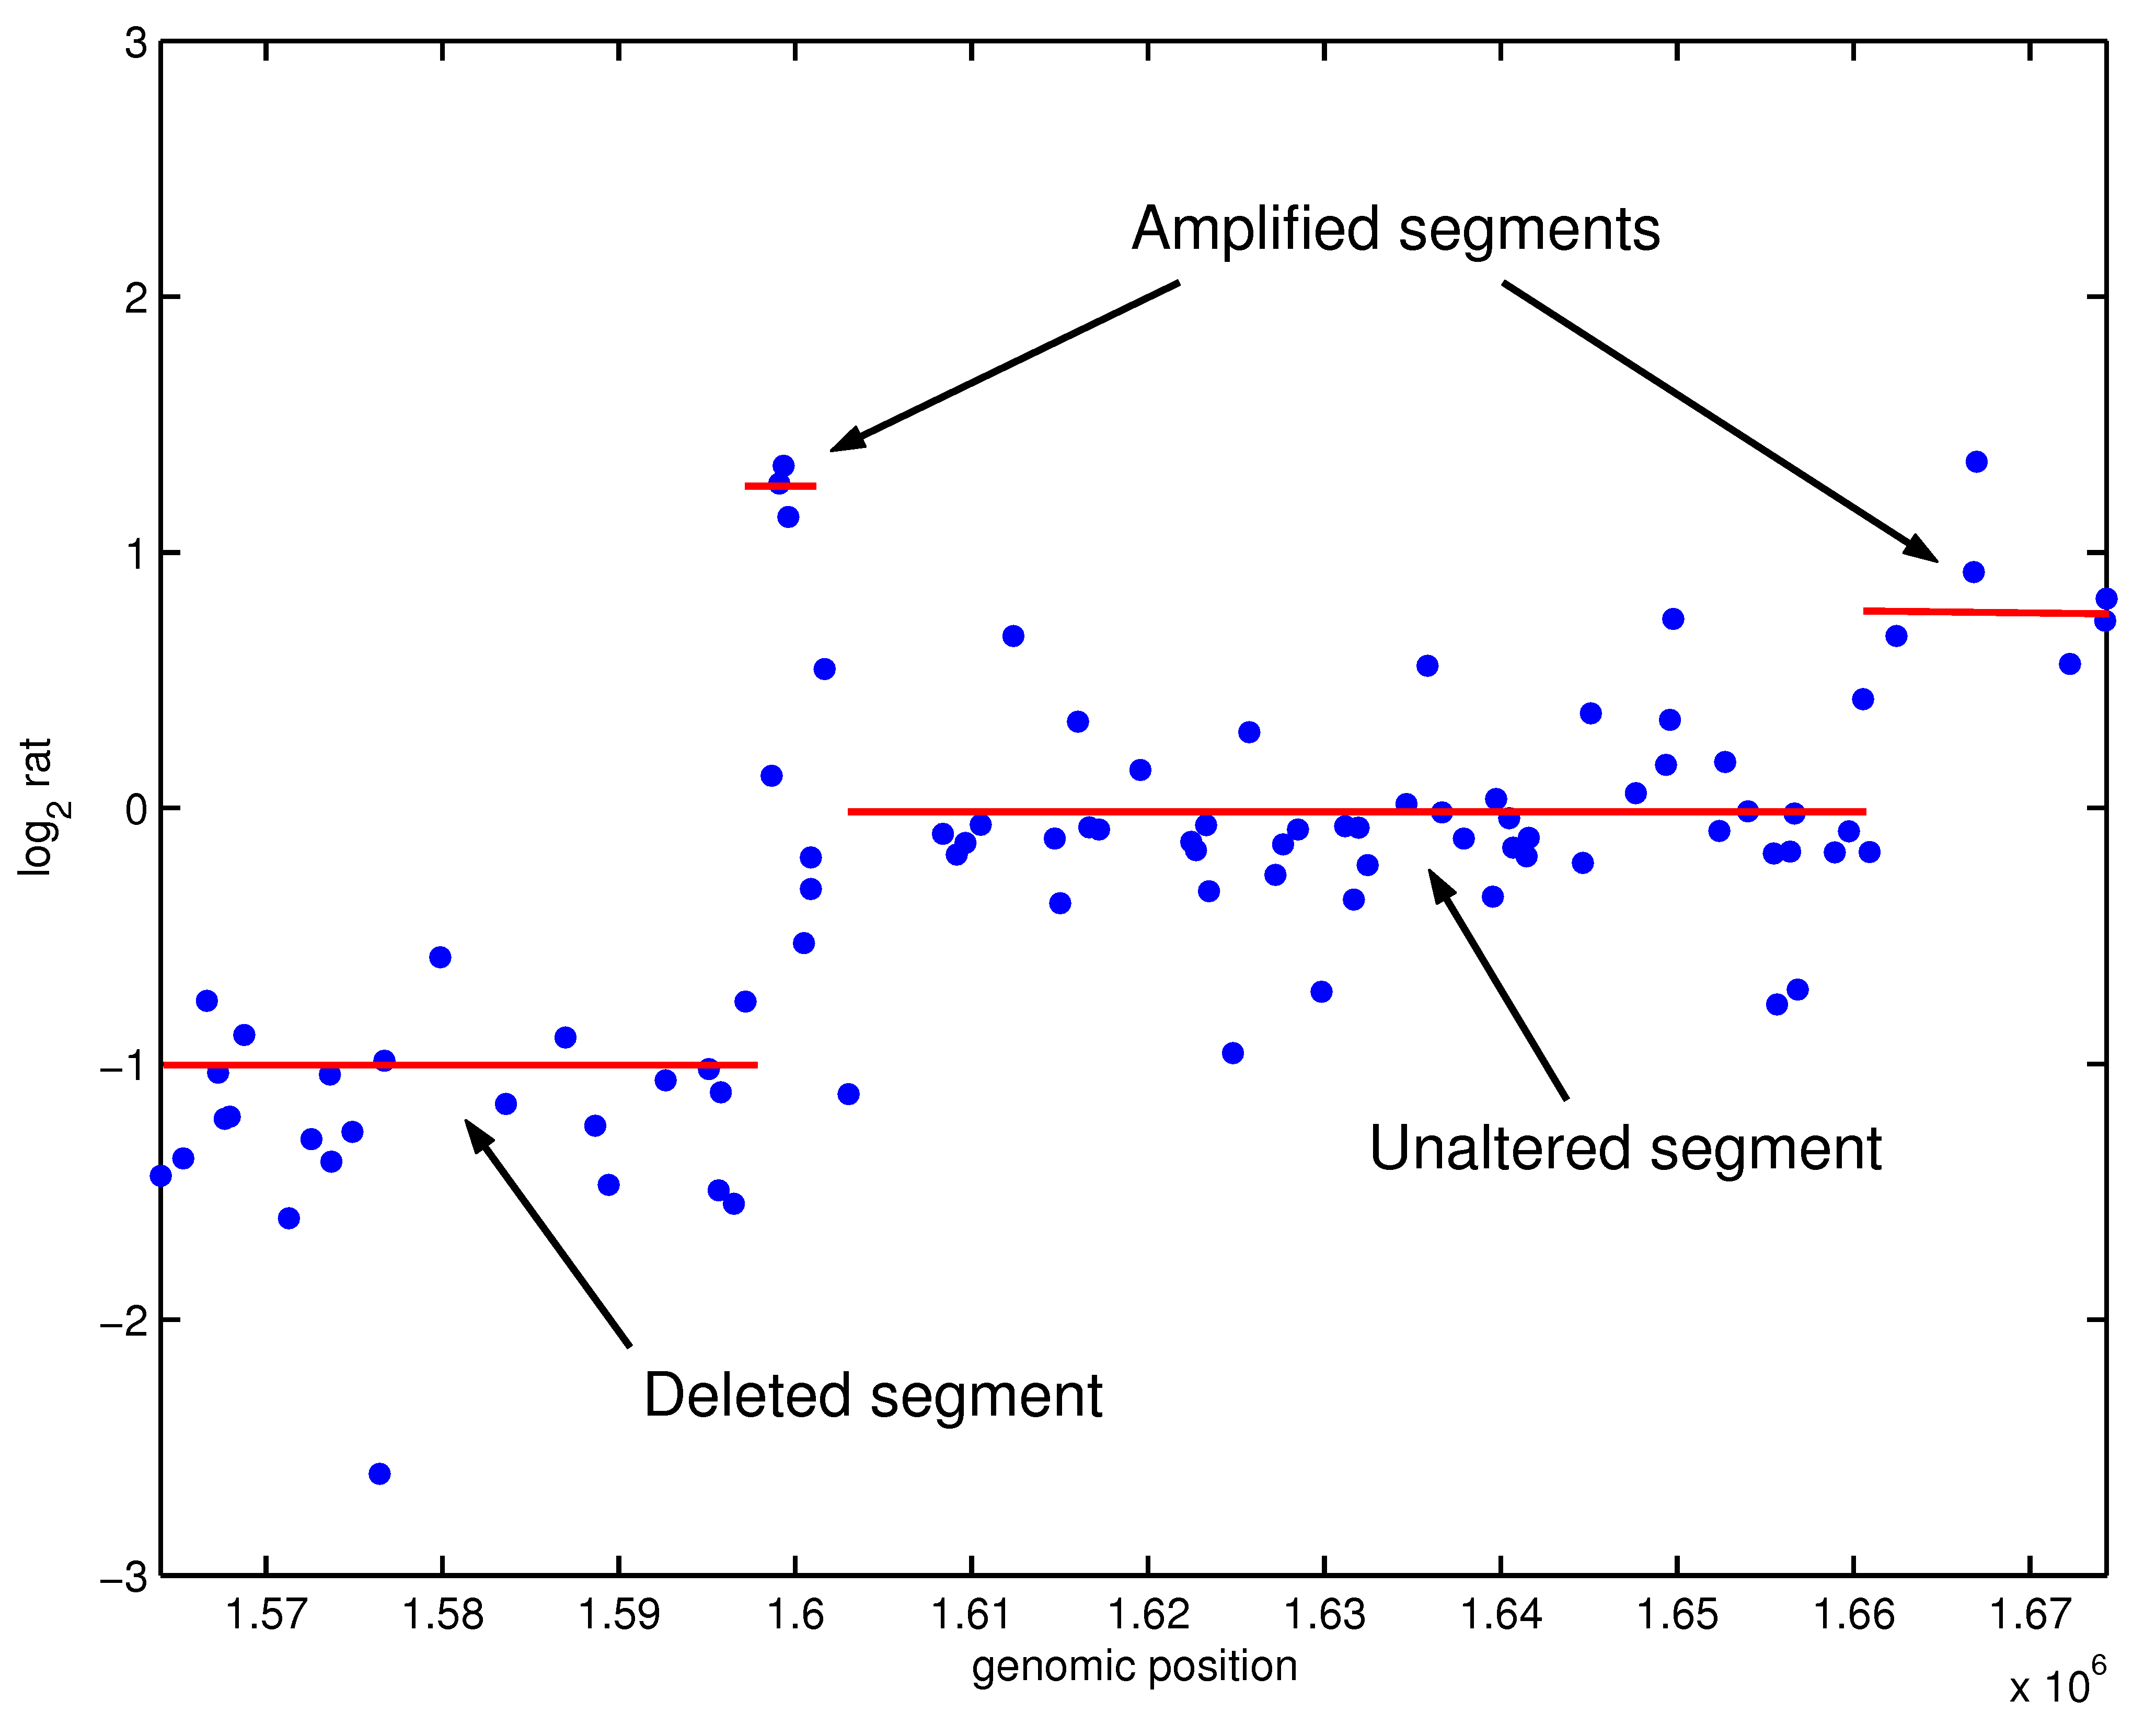
\epsfig{file = ../Figures/profile_example.eps, clip=,
  bbllx=60, bblly=196, bburx=543, bbury=586}
$$

%%%%%%%%%%%%%%%%%%%%%%%%%%%%%%%%%%%%%%%%%%%%%%%%%%%%%%%%%%%%%%%%%%%%%%
\newpage
\begin{enumerate}[$\bullet$]
                                %\vspace{-0.5cm}
\item This classification into \emphase{unknown status} (deleted,
  normal, amplified) can be performed using a \emphase{mixture model}
  for the segments (\emphase{Picard \& al., Biometrics, 07}).
  $$
  \begin{tabular}{cc}
    \paragraph{Segmentation (DP)} & \paragraph{Segmentation /
      Clustering (DP/EM)} \\
    \epsfig{file = ../Figures/FigSegClas-1.eps, clip=, width=10cm, height=7cm} &
    \epsfig{file = ../Figures/FigSegClas-2.eps, clip=, width=10cm, height=7cm}
  \end{tabular}
  $$
\item Segment classification into classes is an \emphase{unobserved
    structure} that has to be recovered. The \emphase{DP/EM
    algorithm} performs simultaneous segmentation and clustering.
\end{enumerate}

%%%%%%%%%%%%%%%%%%%%%%%%%%%%%%%%%%%%%%%%%%%%%%%%%%%%%%%%%%
\newpage
\subsection{Mixture model}
\begin{itemize}
\item We suppose there exists a \textblue{secondary underlying
    structure} of the segments into $P$ populations with weights
  $\pi_1,...,\pi_P (\sum_p \pi_p=1)$.
% \item We introduce hidden variables, $Z_{kp}$ indicators of the
%   population of origin of \textblue{segment $k$}.
% \item Those variables are supposed independent, with multinomial
%   distribution:
%   $$
%   \pi_p = \mbox{proportion of group $p$}
% %   (Z_{k1},\hdots,Z_{kP}) \sim \mathcal{M}(1;\pi_1,\hdots,\pi_P).
%   $$
\item Conditionally to the group to which the segment belongs, we know
  the distribution of $Y$:
  $$
  t \in I_k, k \in p \qquad \Rightarrow \qquad Y_t \sim \Ncal(m_p, s_p^2).
%   Y^k|Z_{kp}=1 \sim \Ncal({\bf 1}_{n_k} m_p, s_p^2 {\bf I}_{n_k}).
  $$
%\item It is a model of \textblue{segmentation/clustering}.
\item The parameters of this model are
  \begin{eqnarray*}
    \mbox{the breakpoint positions:} \quad T&=&(t_1, ..., t_{K-1}),\\
    \mbox{the mixture characteristics:} \quad
    \Theta&=&(\pi_1,\hdots,\pi_P;\theta_1,\hdots,\theta_P), 
    \\
    & & \text{where } \theta_p=(m_p,s_p^2).
  \end{eqnarray*}
\end{itemize}

%%%%%%%%%%%%%%%%%%%%%%%%%%%%%%%%%%%%%%%%%%%%%%%%%%%%%%%%%%
\newpage
\subsection{An hybrid estimation algorithm}
%%%%%%%%%%%%%%%%%%%%%%%%%%%%%%%%%%%%%%%%%%%%%%%%%%%%%%%%%%
%\paragraph{Alternate parameters estimation with $K$ and $P$ known}
\begin{enumerate}
\item When $T$ is fixed, the \textblue{Expectation-Maximization (EM)}
  algorithm estimates $\Theta$:
  $$
  \hat{\Theta}^{(h+1)}=\underset{\Theta}{\arg\max} \left\{\log
    \Lcal_{KP}\left(\Theta,T^{(h)}\right) \right\}. 
  $$
  $$
  \log \Lcal_{KP}( \hat{\Theta}^{(h+1)}; \hat{T}^{(h)})
  \geq \log \Lcal_{KP}(\hat{\Theta}^{(h)};
  \hat{T}^{(h)})
  $$
\item When $\Theta$ is fixed, \textblue{dynamic programming} estimates $T$:
  $$
  \hat{T}^{(h+1)}=\underset{T}{\arg\max} \left\{\log
    \Lcal_{KP}\left(\hat{\Theta}^{(h+1)},T\right) \right\}. 
  $$
  $$
  \log \Lcal_{KP}(\hat{\Theta}^{(h+1)}; \hat{T}^{(h+1)})
  \geq \log \Lcal_{KP}(\hat{\Theta}^{(h+1)};
  \hat{T}^{(h)})
  $$
\end{enumerate} 
\paragraph{An increasing sequence  of likelihoods:}
$$\log \Lcal_{KP}(\hat{\Theta}^{(h+1)}; \hat{T}^{(h+1)}) \geq \log \Lcal_{KP}(\hat{\Theta}^{(h)}; \hat{T}^{(h)})$$

%%%%%%%%%%%%%%%%%%%%%%%%%%%%%%%%%%%%%%%%%%%%%%%%%%%%%%%%%%%%%%%%%%%%%%
\newpage
\paragraph{Application to BT474 cell line, chromosome 1.}
$$
\begin{tabular}{cc}
  Segmentation & Segmentation/Clustering \\
  $K=2$ & $P=3$, $K=8$ \\
  \epsfig{file = ../Figures/bt474_c1_seg_hetero_K2.eps, clip=, scale=0.7} 
  & \epsfig{file = ../Figures/resultat_P3K8.eps , clip=, scale=0.7} 
\end{tabular}
$$
Clustering help in detecting a structure in highly variable
regions.

%%%%%%%%%%%%%%%%%%%%%%%%%%%%%%%%%%%%%%%%%%%%%%%%%%%%%%%%%%%%%%%%%%%%%%
%%%%%%%%%%%%%%%%%%%%%%%%%%%%%%%%%%%%%%%%%%%%%%%%%%%%%%%%%%%%%%%%%%%%%%
\newpage
\section{Future work: Clustering for multiple arrays}
%%%%%%%%%%%%%%%%%%%%%%%%%%%%%%%%%%%%%%%%%%%%%%%%%%%%%%%%%%%%%%%%%%%%%%
%%%%%%%%%%%%%%%%%%%%%%%%%%%%%%%%%%%%%%%%%%%%%%%%%%%%%%%%%%%%%%%%%%%%%%

\begin{enumerate}[$\bullet$]

\item We want to $(i)$ account for correlations between profiles
  ($\Ubf$) , $(ii)$ find the breakpoints ($\Tbf$) and $(iii)$ classify
  segments ($\Cbf$):
  $$
  \Ybf = \Xbf \thetabf + \Tbf \textblue{\Cbf} \mubf + \Zbf \Ubf + \Ebf
  $$
\item We have to recover \emphase{two unobserved informations}: Random
  effects ($\Ubf$) and segment classification ($\Cbf$). \\
  \\
  The maximum likelihood approach leads to \emphase{intractable
    computations} $\Rightarrow$ Standard \emphase{E-M can not be used}.
\item \emphase{Variational approaches} (providing approximate maximum
  likelihood) seem promising.
\end{enumerate}

\bigskip\bigskip 
\centerline{\textred{\framebox{ Post-doc position at AgroParisTech,
    starting this summer (18 months).}}}

%%%%%%%%%%%%%%%%%%%%%%%%%%%%%%%%%%%%%%%%%%%%%%%%%%%%%%%%%%%%%%%%%%%%%%
%%%%%%%%%%%%%%%%%%%%%%%%%%%%%%%%%%%%%%%%%%%%%%%%%%%%%%%%%%%%%%%%%%%%%%
%%%%%%%%%%%%%%%%%%%%%%%%%%%%%%%%%%%%%%%%%%%%%%%%%%%%%%%%%%%%%%%%%%%%%%
%%%%%%%%%%%%%%%%%%%%%%%%%%%%%%%%%%%%%%%%%%%%%%%%%%%%%%%%%%%%%%%%%%%%%%
\end{document}
%%%%%%%%%%%%%%%%%%%%%%%%%%%%%%%%%%%%%%%%%%%%%%%%%%%%%%%%%%%%%%%%%%%%%%
%%%%%%%%%%%%%%%%%%%%%%%%%%%%%%%%%%%%%%%%%%%%%%%%%%%%%%%%%%%%%%%%%%%%%%
%%%%%%%%%%%%%%%%%%%%%%%%%%%%%%%%%%%%%%%%%%%%%%%%%%%%%%%%%%%%%%%%%%%%%%
%%%%%%%%%%%%%%%%%%%%%%%%%%%%%%%%%%%%%%%%%%%%%%%%%%%%%%%%%%%%%%%%%%%%%%

